\documentclass[letterpaper]{article}
\usepackage{amsmath}
\usepackage{tikz}
\usepackage{epigraph}
\usepackage{lipsum}
\usepackage{hyperref}
\usepackage{tocloft}
\usepackage{graphicx}
\usepackage{float}

\usepackage{setspace, amsmath}

\usepackage[centering,includeheadfoot,margin=2cm]{geometry}
\usepackage{xcolor}
\usepackage{calc,blindtext}

\renewcommand\epigraphflush{flushright}
\renewcommand\epigraphsize{\normalsize}
\setlength\epigraphwidth{0.6\textwidth}

\definecolor{titlepagecolor}{cmyk}{1,.60,0,.40}

\DeclareFixedFont{\titlefont}{T1}{ppl}{b}{it}{1.0in}

\makeatletter
\def\printauthor{%
    {\large \@author}}
\makeatother
\author{%
    Nico Taljaard \\
    10153285 \vspace{20pt} \\
    Gerhard Smit \\
    12282945 \vspace{20pt} \\
    Martin Schoeman \\
    10651994 \\
}

% The following code is borrowed from: http://tex.stackexchange.com/a/86310/10898

\newcommand\titlepagedecoration{%
	\begin{tikzpicture}[remember picture,overlay,shorten >= -10pt]
	
		\coordinate (aux1) at ([yshift=-15pt]current page.north east);
		\coordinate (aux2) at ([yshift=-410pt]current page.north east);
		\coordinate (aux3) at ([xshift=-4.5cm]current page.north east);
		\coordinate (aux4) at ([yshift=-150pt]current page.north east);
		
		\begin{scope}[titlepagecolor!40,line width=12pt,rounded corners=12pt]
			\draw
			  (aux1) -- coordinate (a)
			  ++(225:5) --
			  ++(-45:5.1) coordinate (b);
			\draw[shorten <= -10pt]
			  (aux3) --
			  (a) --
			  (aux1);
			\draw[opacity=0.6,titlepagecolor,shorten <= -10pt]
			  (b) --
			  ++(225:2.2) --
			  ++(-45:2.2);
		\end{scope}
			\draw[titlepagecolor,line width=8pt,rounded corners=8pt,shorten <= -10pt]
			  (aux4) --
			  ++(225:0.8) --
			  ++(-45:0.8);
		\begin{scope}[titlepagecolor!70,line width=6pt,rounded corners=8pt]
			\draw[shorten <= -10pt]
			  (aux2) --
			  ++(225:3) coordinate[pos=0.45] (c) --
			  ++(-45:3.1);
			\draw
			  (aux2) --
			  (c) --
			  ++(135:2.5) --
			  ++(45:2.5) --
			  ++(-45:2.5) coordinate[pos=0.3] (d);   
			\draw 
			  (d) -- +(45:1);
		\end{scope}
	\end{tikzpicture}
}

\begin{document}

\begin{titlepage}

\noindent
\titlefont Laminin \par
\epigraph{ XGame - Derivco \\ Corspe Slasher \\ Software Architecture Specification}%
{\textit{ 01/08/2014 }\\ \textsc{ }}
\null\vfill
\vspace*{4cm}
\noindent
\hfill
\begin{minipage}{0.35\linewidth}
    \begin{flushright}
        \printauthor
    \end{flushright}
\end{minipage}
%
\begin{minipage}{0.02\linewidth}
    \rule{1pt}{125pt}
\end{minipage}
\titlepagedecoration
\end{titlepage}

% % % % % % % % % % % % % % %
% 							%
%	Remainder of document	%
% 							%
% % % % % % % % % % % % % % % 

	\newpage
		{\LARGE \bf Change Log}\\[2em]
		
		\begin{tabbing}
			\hspace*{2.5cm}\=\hspace*{2.5cm}\=\hspace*{8cm}\=\hspace*{3cm} \kill
   			17/05/2014	\> Version 1.0	\> Document Created 							\> Nico Taljaard \\
			19/05/2014  \> Version 1.0  \> Added Vision									\> Martin Schoeman \\
			21/05/2014  \> Version 1.0  \> Added High Level Use Case Diagram			\> Martin Schoeman\\
			22/05/2014  \> Version 1.0  \> Added Sub Level Use Case Diagram				\> Martin Schoeman\\
			23/05/2014  \> Version 1.0  \> Corrected Page Format						\> Martin Schoeman \\
			23/05/2014  \> Version 1.0  \> Added Title Page Information					\> Martin Schoeman \\
			23/05/2014  \> Version 1.0  \> Added Limitations \& Exclusions				\> Martin Schoeman \\
			30/07/2014	\> Version 1.0	\> Added document factors						\> Nico Taljaard \\
			01/08/2014	\> Version 1.0	\> Added quality requirements					\> Nico Taljaard \\
			01/08/2014	\> Version 1.0	\> Added technologies							\> Nico Taljaard \\
			01/08/2014	\> Version 1.0	\> Added tactics and strategies					\> Nico Taljaard \\
			09/09/2014	\> Version 1.0	\> Updated quality requirements					\> Nico Taljaard \\
			10/09/2014 	\> Version 1.0  \> Added higher level use case diagram			\> Martin Schoeman\\
			10/09/2014  \> Version 1.0	\> Moved architectural constraints to technology\> Martin Schoeman\\
			10/09/2014  \> Version 1.0  \> Inserted correct architectural constraints	\> Martin Schoeman\\
			10/09/2014	\> Version 1.0  \> Added a security quality requirement			\> Martin Schoeman\\
			10/09/2014	\> Version 1.0	\> Update patterns \& strategies				\> Gerhard Smit \\
			10/09/2014	\> Version 1.0	\> Simpe UI use case							\> Gerhard Smit \\
			11/09/2014	\> Version 1.0	\> Spacing changes								\> Nico Taljaard \\
			01/10/2014	\> Version 2.0	\> Extended frameworks used.					\> Nico Taljaard \\
			01/10/2014	\> Version 2.0	\> Added community contribution.				\> Nico Taljaard \\
			01/10/2014	\> Version 2.0	\> Added technology limitations.				\> Nico Taljaard \\
			02/10/2014	\> Version 2.0	\> Added java server limitations.				\> Martin Schoeman\\
			02/10/2014	\> Version 2.0	\> Added overcoming server limitations.			\> Martin Schoeman\\
			03/10/2014	\> Version 2.0	\> Added Nifty GUI limitations.				\> Gerhard Smit\\
			03/10/2014	\> Version 2.0	\> Added overcoming Nifty GUI limitations.			\> Gerhard Smit\\
		\end{tabbing}
		
	\newpage
		\renewcommand\contentsname{TABLE OF CONTENTS}
		\newcommand\contentsnameLC{\colorbox{blue}{\makebox[\textwidth-2\fboxsep][l]{\bfseries\color{white} Table of Contents}}}
		
		\renewcommand{\cftdot}{}
		\hypersetup{linktocpage}
		\tableofcontents
		
		\begin{flushleft}
			\LARGE\href{https://github.com/njTaljaard/Laminin_CorpseSlasher/}{Git repository: Laminin - Corpse Slasher}
		\end{flushleft}
		
	\newpage
	
		\section*{\colorbox{blue}{\makebox[\textwidth-2\fboxsep][l]{\bfseries\color{white} Vision }}} \addcontentsline{toc}{section}{Vision}
		\vspace{0.2in}
		
		The vision of this project is to create a game that supports multiple platforms, for example android devices and windows computers. The game should be connected to a server where game data can be saved and retrieved real time. The user should be able to log in using a custom log in or an OAuth log in that uses social media like Facebook and Google+. There must also be a live leader board and achievements. It must be able to develop the game in three months. The project must be developed using only open source and freeware technologies.
					
		\section*{\colorbox{blue}{\makebox[\textwidth-2\fboxsep][l]{\bfseries\color{white} Scope}}} \addcontentsline{toc}{section}{Scope}
		
		\vspace{0.2in}
		
		\begin{figure}[ht!]
		\centering
		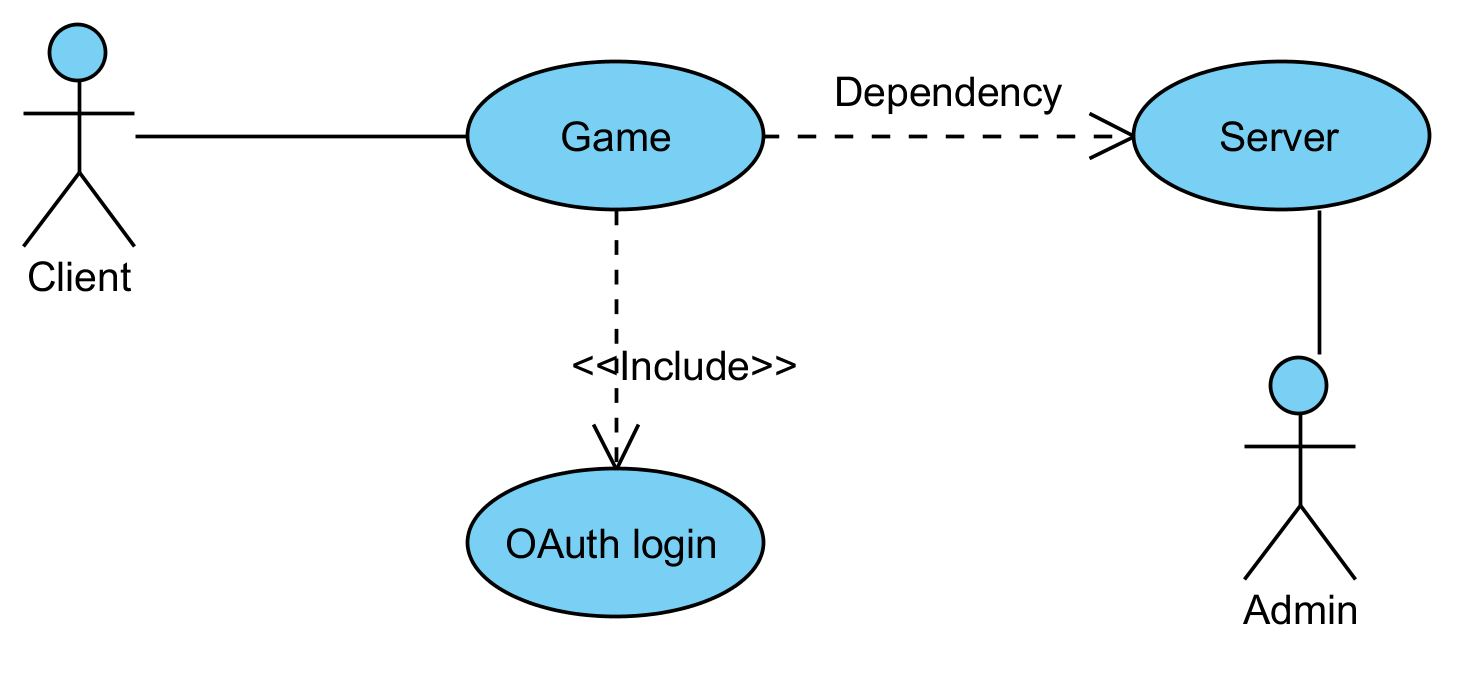
\includegraphics[width=180mm, height=50mm]{UML_Diagram/Use_Case/High_Level}
		\caption{High level use case diagram}
		\label{overflow}
		\end{figure}
		
		\begin{figure}[H]
		\centering
		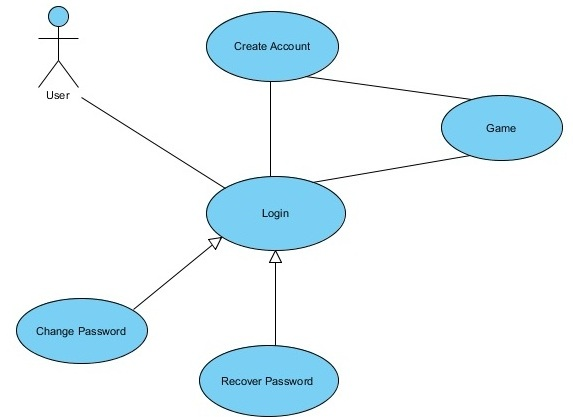
\includegraphics[width=180mm, height=70mm]{UML_Diagram/Use_Case/login_simple}
		\caption{Login use case diagram}
		\label{overflow}
		\end{figure}		
				
		\vspace{0.2in}
		
		\section*{\colorbox{blue}{\makebox[\textwidth-2\fboxsep][l]{\bfseries\color{white} Sub-level use case diagrams}}} \addcontentsline{toc}{section}{Sub-level use case diagrams}
				
		\begin{figure}[ht!]
		\centering
		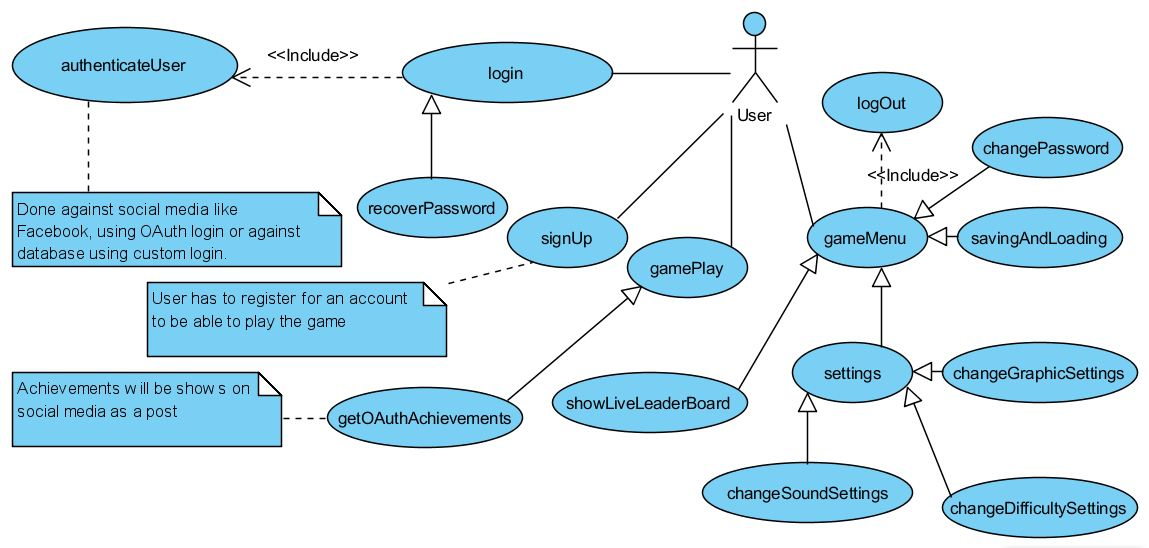
\includegraphics[width=180mm]{UML_Diagram/Use_Case/high_level_use_case_diagram}
		\caption{High level use case diagram for game}
		\label{overflow}
		\end{figure}
		
		\vspace{0.2in}
		
		\begin{figure}[ht!]
		\centering
		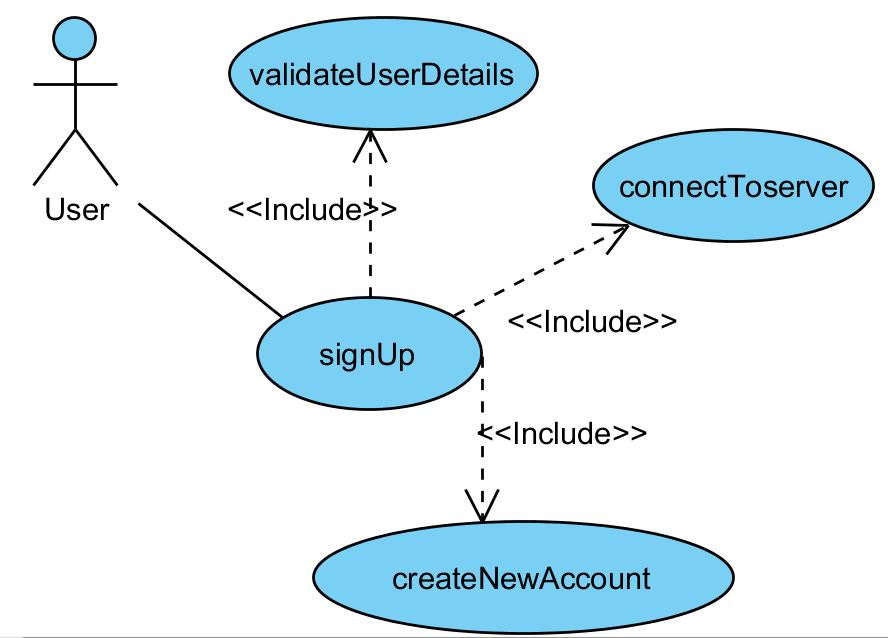
\includegraphics[width=180mm, height=70mm]{UML_Diagram/Use_Case/signup}
		\caption{Sign up use case diagram}
		\label{overflow}
		\end{figure}
		
		\vspace{0.2in}
		
		\begin{figure}[H]
		\centering
		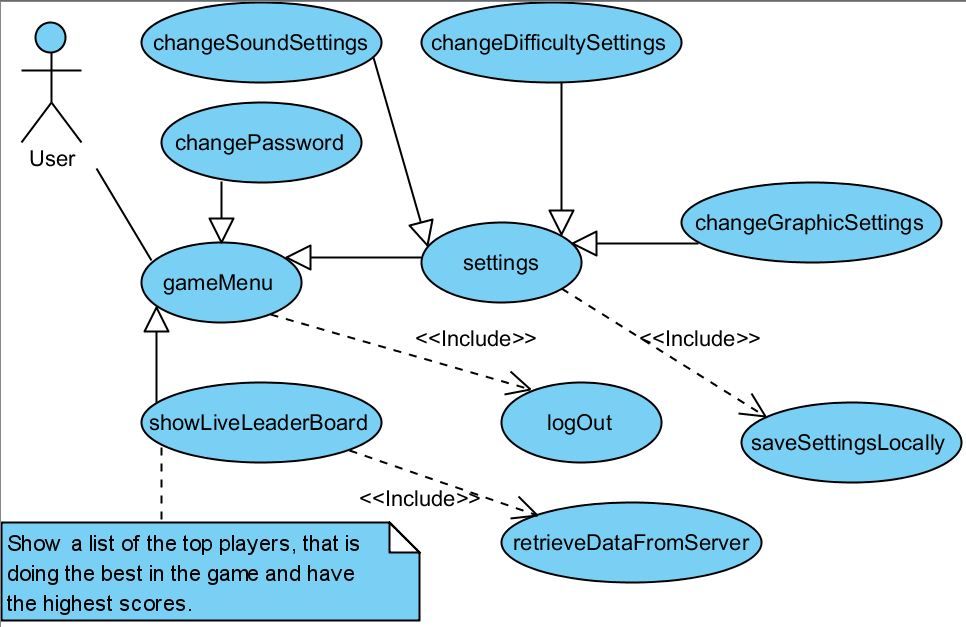
\includegraphics[width=180mm]{UML_Diagram/Use_Case/game_menu}
		\caption{Game menu use case diagram}
		\label{overflow}
		\end{figure}
		
		\section*{\colorbox{blue}{\makebox[\textwidth-2\fboxsep][l]{\bfseries\color{white} Limitations \& Exclusions}}} \addcontentsline{toc}{section}{Limitations \& Exclusions}
		\vspace{0.2in}
		
		\begin{itemize}
  		\item Download, we only have to develop the game. We have no responsibility of distribution.
  		\item Install, we are not responsible for the development of an installer.
  		\item Compatibility, the game will not necessarily work with all hardware.
  		\item Game engine itself has performance limitation where it does not use all available resources.
  		\item The game should be able to run on mobile and desktop. This leads to having lower performance settings on android then on desktop.
  		\item There is no requirement for having multiple maps or enemies.
  		\item Social OAuth login is only required for Facebook and Google+.
		\end{itemize}
		
		\section*{\colorbox{blue}{\makebox[\textwidth-2\fboxsep][l]{\bfseries\color{white} Architectural requirements }}} \addcontentsline{toc}{section}{Architectural requirements}
		\vspace{0.1in}
			
			\subsection*{ Architectural scope }
			\addcontentsline{toc}{subsection}{Architectural scope}
			\vspace{0.1in}	
			We will be providing a persistance infrastructure in the form of a database which will allow us to store user information such as email addresses, usernames, passwords and game information i.e. Character location, Health and Experience. There will be a reporting infrastructure between the client and the server for updating the leaderboard, to display the progress of multiple users. As a nice to have we would like to add another reporting infrastructure on the server side to allow for printing of graphs related to client logging and more. There is an infrustracture in place for process execution which controls the frame updates, user-interfaces being called at the appropriate times also there are server side process execution infrastructures handled purely by the server, which sends and receives data from the client also sending through an email to the user with password details. There is a login infrastructure in place using social media (OAuth) to login or a custom login where an account is required. 
				
			\vspace{0.2in}
			\subsection*{ Quality requirements }
			\addcontentsline{toc}{subsection}{Quality requirements}
			\vspace{0.1in}
				
				The quality requirements are the requirements around the quality attributes of the systems and the
				services it provides.
				
				\subsubsection*{Performance}
				\addcontentsline{toc}{subsubsection}{Performance}
				\vspace{0.1in}
				
					\begin{itemize}
						\item Desktop \& Mobile application:
							\begin{itemize}
								\item Should not go under a playable frames rate of 60: \\
										Reduce polygon count.
								\item Should not require a high speed internet connection more then 2Mbit/sec: \\
										No large date will be sent requiring faster line speeds.
								\item Should not send more then 100Kb/min: \\
										Only use the connection for updating kills, and login.
								\item Should not require more the 4 logical processing cores: \\
										Limit the need to access cpu and split processing among cores.
							\end{itemize}
							
						\item Desktop application:
							\begin{itemize}
								\item Should not use more the 3GB of system memory: \\
										Limit variable and model creation.
								\item Should not require more then 1GB of VRAM: \\
										Limit vertex count.
								\item Should not require higher then 2.0 GHz system processor: \\
										Limit processes designated to cpu during frame update.
								\item Should not require higher then 500 MHz gpu processor: \\
										Limit game effects and processes per frame.
							\end{itemize}
							
						\item Mobile application:
							\begin{itemize}
								\item Should not use more the 1GB of system memory: \\
										Reduce variable and vertex count for entire game.
								\item Should not use access battery usage: \\
										Do not over use system resources requiring more reads and writes to memory.
								\item Should not require higher then a 1.0 GHz system: \\
										Reduce cpu processes from desktop version.
							\end{itemize}
							
						\item Backend server:
							\begin{itemize}
								\item Should be able to handle at least 100 connections: \\
										Using a thread pool manager.
								\item Should not use more then 10GB of system memory to handle connections: \\
										Limit variable creation per thread.
								\item Database updates should be complete within a 0.1 second time frame: \\
										Database manages thread pooling for connections.
								\item Database requests should be complete within 0.5 second time frame: \\
										Optimize requests for optimal database processing. 
							\end{itemize}
					\end{itemize}
				
				\subsubsection*{Reliability}
				\addcontentsline{toc}{subsubsection}{Reliability}
				\vspace{0.1in}
				
					\begin{itemize}
						\item Desktop \& Mobile:
							\begin{itemize}
								\item Client should be able to recover from a crash within 30 seconds: \\
										Retry for re-establishing server connection.
								\item Retry opening connection within 5 seconds if connection loss.
								\item Reload assets if data is lost.
							\end{itemize}
						\item Backend Server:
							\begin{itemize}
								\item Should provide 99\% connection availability: \\
										Exception handling to prevent the server from crashing and recovery from errors.
								\item Should provide 99\% OAuth login availability through SocialAuth: \\
										Up to social media server up time.
								\item Should not crash due to over welling client connections: \\
										Managed by thread pooling.
								\item Should not crash due to undefined incoming data: \\
										Input is checked and filtered before processing.
								\item Should not drop connections due to inactivity or data loss: \\
										Thread pool controls live time of thread.
							\end{itemize}
					\end{itemize}
					
				\subsubsection*{Scalability}
				\addcontentsline{toc}{subsubsection}{Scalability}
				\vspace{0.1in}
					
					\begin{itemize}
						\item Game
							\begin{itemize}
								\item Adding multiple maps for game play as a nice to have: \\
										Add the selection UI and file name containing scene.
								\item Adding a variety of enemy players as a nice to have.
								\item Adding further environmental features as a nice to have. \\ \\
							\end{itemize}
						\item Backend Server:
							\begin{itemize}
								\item The server should be able to add multiple servers to handle clients as a nice to have: \\
									Add multiple IP and/or sockets which to attempt connecting to remove center point of failure.
								\item The server should scale to any amount of client connections, with an improved system performance: \\
									Add multiple servers through horizontal scaling, or vertical scaling having more threads and memory to process threads.
							\end{itemize}
					\end{itemize}
				
				\subsubsection*{Security}
				\addcontentsline{toc}{subsubsection}{Security}
				\vspace{0.1in}
				
					General security conditions.
					\begin{itemize}
						\item Use OAuth LDAP for connection to social media e.g. Facebook, Google+.
						\item Password encryption on database side as well as when signing in through custom loggin.
						\item Password retrieval only to an know uses with a verified email address.
						\item Clean up all incoming data on client and server for incorrect formats, data types \& lengths.
						\item Test if the incoming data comes from authenticated user.
						\item Encrypt all passwords sent from client to server and no passwords ever gets sent from server to client, unless it is to their email address.
					\end{itemize}
				
				\subsubsection*{Maintainability}
				\addcontentsline{toc}{subsubsection}{Maintainability}
				\vspace{0.1in}
				
					\begin{itemize}
						\item Database off site backups should be creatable as a nice to have: \\
								Export the entire database for backup.
						\item Update look and feel of user interface as nice to have.
						\item Update versions of libraries as nice to have, social media security access updates need to be changed within is code.
						\item Change models to higher resolution textures.
					\end{itemize}
				
			\vspace{0.2in}
			\subsection*{ Integration and access channel requirements }
			\addcontentsline{toc}{subsection}{Integration and access channel requirements}
			\vspace{0.1in}
			
				\hspace{5mm}Integration channels:
					\begin{itemize}
						\item Server needs to connect to MySQL database.
						\item We use SMTP to send out mails.
						\item We use HTTP to do the OAuth authorization.
						\item We use TCP/IP to connect client to server and exchange data between client and server.
						\item We use Nifty GUI to display GUI's in the game.
					\end{itemize}
				
				\newpage			
				
				The system will be accessible by human users through the following channels:
				\begin{itemize}
					\item From a desktop application running on any Windows/Linux operating system.
					\item From a mobile device running Android application clients.
					\item From social media like Facebook and Google+.
				\end{itemize}
				
				The system will be accessible by other systems through the following channels:
				\begin{itemize}
					\item OAuth authorization with Facebook and Google+.
					\item Gmail, sending out emails.
				\end{itemize}
				
			\vspace{0.2in}
			\subsection*{ Architectural constraints }
			\addcontentsline{toc}{subsection}{Architectural constraints}
			\vspace{0.1in}
					\vspace{0.1in}
		
			
				\begin{enumerate}
					\item \textbf{Open source}
					\\Research open source or freeware technologies available; this includes freely available art work.
					
					\item \textbf{Cross-platform}
					\\The game needs to run on at least two different platforms (desktop and mobile) or can be an HTML application that can be wrapped for different platforms.
					
					\item \textbf{Using OAuth login and posts}
					\\OAuth integration; Facebook, Twitter or G+ login and achievement updates.
					
					\item \textbf{Custom login}
					\\if user does not want to use OAuth, he or she can use custom login.
					
					\item \textbf{Encryption}
					\\Passwords needs to be encrypted when stored.
					
					\item \textbf{Recover password}
					\\Add forgot password feature.
									
					\item \textbf{Live Leader Board}
					\\The game needs to have a points system that updates real time.
					
					
				\end{enumerate}
			
		\vspace{0.2in}
			
			
			
		\vspace{0.2in}
		\section*{\colorbox{blue}{\makebox[\textwidth-2\fboxsep][l]{\bfseries\color{white} Architectural patterns or styles }}}
		\addcontentsline{toc}{section}{Architectural patterns or styles}
		\vspace{0.1in}
		\begin{itemize}
		\item Game :
		\begin{itemize}
		\item Concurrency : All the mobs that are in the update radius are updated per frame to a new position, state or animation.
		\item Queuing : The thread pooling in place makes use of a blocking queue.
		\item Layering : The game/client side makes use of a layering system through the update, where a game update occurs and then the update is sent to the character and mod handler to update their respective locations or states.
		\item Interpreter : The opening of user-interface screens are being sent to a single class to open the correct screen.
		\item Iterator : When an update to the size of the user-interface is being made all the screens are updated in succession.
		\end{itemize}
		\item Server :
		\begin{itemize}
		\item Facade : There is a single input class that acts as in interface for all the server classes.
		\item Interpreter : There is a single input class redirecting all the commands coming from the client to the different server classes.
		\item Layering : Multiple layers have been implemented on the server side, to allow for better security and simplicity.
		\item Blackboard system : The oauth classes posts on the user's social media page on his behalf.
		\item Event-drive : When a server call or event is requested from the client side, the server processes that query that was sent. 
		\item MVC : The client connection is the view, server is the controller and the database is the model.
		\item Multitier : The structure that exists between the client and the server.
		\item Pipe and filter : The connection between the server and the client is the pipe while the server itself acts as the filter.
		\item Service orientated : There are multiple plugable aspects regarding the server such as the ability to send emails and the database being used.
		\end{itemize}
		\end{itemize}
		\vspace{0.2in}
		\section*{\colorbox{blue}{\makebox[\textwidth-2\fboxsep][l]{\bfseries\color{white} Architectural tactics or strategies }}}
		\addcontentsline{toc}{section}{Architectural tactics or strategies}
		\vspace{0.1in}
			
			\begin{itemize}
				\item Game:
					\begin{itemize}
						\item Low poly models are used to reduce the gpu processing to calculate each points position and colour and display it and vram space required to store each points data.
						\item Low amount of enemies to reduces processing requirements.
						\item Adding hills on the terrain to simplify graphic calculation to shorten distance rendering.
						\item Simplify collision boxes to ease the calculations done by Bullet Physics.
						\item Designing a single map, due to having multiples are repeating completed work. Adding more are nice to have.
						\item Using a single enemy model due to time constraint for creating multiple models and animating them.
						\item Single user-interface display which multiple screens can couple to.
					\end{itemize}
				\item Server:
					\begin{itemize}
						\item Thread pooling is implemented by Java thread pool executor for all incoming connections so that each thread has sufficient time for CPU access and no dead lock can occur because each thread runs on each own instance of the server.
						\item Reopening JDBC for each request to free up memory space and cpu cycles.
					\end{itemize}
			\end{itemize}
			
		\vspace{0.2in}
		\section*{\colorbox{blue}{\makebox[\textwidth-2\fboxsep][l]{\bfseries\color{white} Use of reference architectures and frameworks }}}
		\addcontentsline{toc}{section}{Use of reference architectures and frameworks}
		\vspace{0.1in}
			
			\begin{itemize}
				\item jMonkeyEngine is a Java SDK framework that is used as our game engine. The engine is in control of communications to OpenGL for rendering, frame updates, loading required assets, accessing model animations to be ran through programming. This framework was chosen for it use of Java which is known by all group members, the ease of use and stability of Java over C++ We did not want to go for a well known open source game engine to have a bit of a challenge also to have a chance to contribute to the community.
				\item BulletPhysics used for game physics, it will control the world gravity, world collision, custom collision defined for each model, ghost collision for proximity detection, attack collision for player sword and model hand to be able to detect when an attack has successfully landed, rag doll physics for death scene.
				\item OAuth as a standard for connection to social media. It insurers a secure connection to login using your social login to obtain data and post data on behalf of the user. This is needed to add the users to the database who wish to login via social media to keep track of their experience.
				\item NiftyGUI is an easy library for creating and updating the user-interface aspect of the game. It has built in functionality for creating the interfaces and action listeners for user interaction. This library was used as it was easy to learn and it was widely supported, it also had multiple ways of creating GUIs through the use of the Java API or through an XML document.
			\end{itemize}
			
		\vspace{0.2in}
		\section*{\colorbox{blue}{\makebox[\textwidth-2\fboxsep][l]{\bfseries\color{white} Access and integration channels }}}
		\addcontentsline{toc}{section}{Access and integration channels}
		\vspace{0.1in}
			
			\begin{itemize}
				\item Human access channels:
					\begin{itemize}
						\item Web services, like web browsers for Facebook and Google+ OAuth authorization.
						\item Mobile front-end, like tablets and smart phones for game play.
						\item Web services, when receiving emails from server.
						\item Desktop for game play.
					\end{itemize}
				\item System access channels:
					\begin{itemize}
						\item Web services to send email using gmail.
						\item Web services to communicate with Facebook and Google+.
					\end{itemize}
				\item Integration channels: \\
					  \begin{itemize}
						\item MySQL database to access stored data.
						\item Web services to communicate between client and server.
						\item Nifty GUI for displaying menus.
						\item OAuth authorization to communicate with social media.
					\end{itemize}
			\end{itemize}
			
		\vspace{0.2in}
		\section*{\colorbox{blue}{\makebox[\textwidth-2\fboxsep][l]{\bfseries\color{white} Technologies }}}
		\addcontentsline{toc}{section}{Technologies}
		\vspace{0.1in}
		
		\begin{enumerate}					
					\item \textbf{Graphics}
					\\OpenGL 2.0 - 4.4 / OpenES 2.0+ will be used as the rendering language within the game engine, it is an open source graphical language allowing for rendering.
					
					\item \textbf{Audio}
					\\OpenAL 1.0 will be used for audio within the game, it is an open source audio language allowing for audio rendering.
					
					\item \textbf{Development language}
					\\The desktop \& mobile application as well as the server will be implemented using JavaSE as it is a widely supported language and has a powerful API with a huge support community, Java is also compatiable with the Android platform and it is easy to integrate between Android and Java as Android is based on Java.
					
					\item \textbf{LDAP integration}
					\\Apache oltu is a Java implemented OAuth(version 1.0) library that will be the used to communicate with external LDAP servers. LDAP is a safe and secure database service that will prevent access to unwanted users. SocialAuth is easy to use and widely supported and very simple to understand.
					
					\item \textbf{Networking}
					\\jSpiderMonkey will be used to handle client side networking within the jMonkeyEngine framework as a nice to have for later purposes of multiplayer functionality as nice to have.
					
					\item \textbf{Persistence}
					\\MySQL will be used to store all data which is accessible through a JDBC. MySQL is easy to use and very powerful as it allows for over 100000 concurrent connections at a time, it has a huge support community, it is also very easy to intergrate with Java.
				\end{enumerate}
			
			\begin{itemize}
				\item Game:
					\begin{itemize}
						\item Java for all programming purposes.
						\item OpenGL \& ES for graphics rendering.
						\item OpenAL for audio.
						\item Blender for model creation, texturing, rigging and animations.
					\end{itemize}
				\item Server:
					\begin{itemize}
						\item Java for all programming purposes.
						\item JSON for data transfer objects.
						\item HTTP connection between server and desktop \& mobile game.
						\item STMP for password recovery.
					\end{itemize}
				\item Operating system: \\
					  Windows 7 \& 8, Andriod 2.2+
			\end{itemize}
			
		\vspace{0.2in}
		\section*{\colorbox{blue}{\makebox[\textwidth-2\fboxsep][l]{\bfseries\color{white} Technology Limitations }}}
		\addcontentsline{toc}{section}{Technology Limitations}
		\vspace{0.1in}
				
			\begin{enumerate}
				\item jMonkey to desktop:
					\begin{itemize}
						\item jMonkey does not use all available graphics processing power. This results in lower frames per second then expected.
						\item Support for positional audio, to change volumes depending on player position. \\
					\end{itemize}
				
				\item jMonkey to Android:
					\begin{itemize}
						\item Creating a scene in the scene composer and loading into Android does not load textures with.
						\item Textures do not load correctly with models.
						\item Ghost collision boxes does not detect any collision or overlapping of other collision boxes.
						\item JoyStick events are not created to be used for Android requires TouchEvent to processes camera and movement.
						\item Frame limitation of 60 frames per second. \\
					\end{itemize}
				
				\item Nifty GUI when using Java:
					\begin{itemize}
						\item Can not change text sizes but is available through XML.
						\item Can not change fonts but is available through XML.
					\end{itemize}
					
					\item Java Server and client connection:
					\begin{itemize}
						\item Server can only communicate with client and vice versa using string values. 
					\end{itemize}
					\item Java threads writing to file:
					\begin{itemize}
						\item When threads write to the audit and error logs, only one thread can write to the file at a time. That causes a bottle neck. 
					\end{itemize}
			\end{enumerate}
				
		\vspace{0.2in}
		\section*{\colorbox{blue}{\makebox[\textwidth-2\fboxsep][l]{\bfseries\color{white} Overcoming limitations }}}
		\addcontentsline{toc}{section}{Overcoming limitations}
		\vspace{0.1in}	
			
			\begin{enumerate}
				\item Game:
				
				\item UI: \item There is no work around for this issue of the font and text size not being adjustable through Java, a look at moving over to another Library in the future is the best solution.
				
				\item Server:
					\begin{itemize}
						\item Format the string values to a JSON object(which is a normal string that is in the JSON format). All passwords are encrypted that is sent from client to server.
					\end{itemize}
					\begin{itemize}
						\item Use the main class to write to the audit and error log files. Because the main class is a static class and only uses one thread, all the threads can call the main's functions to write to the logs for them. Seeing as the main class is the only one writing to the files, the main can keep the files open and does not have to worry about other threads wanting access to the files. You can see this method as making your main class the "queue" for all the thread's errors and audits that needs to be written to the files. 
					\end{itemize}
			\end{enumerate}
				
		\vspace{0.2in}
		\section*{\colorbox{blue}{\makebox[\textwidth-2\fboxsep][l]{\bfseries\color{white} Community contribution }}}
		\addcontentsline{toc}{section}{Community contribution}
		\vspace{0.1in}
			
			\begin{itemize}
				\item A null pointer that can exist at not expected moments when using the build in Ragdoll class. When using the Ragdoll in combination with BetterCharacter control you can not use all the facets of the Ragdoll which caused this problem. This was solved by removing unwanted functionality when using the BetterCharacter control for motion control.
				\item No support exists for automatic detection of the SkeletonController or AnimationController when it does not reside in the root node of the used model. A recursive function was created that will traverse the children nodes until the required controller is found. This removes the need of hard coding where to find the controllers for each model used.
			\end{itemize}
\end{document}